% Généré par md2tex.py — ne pas éditer à la main ; éditer le .md maître et reconvertir.
% Compile : pdflatex (deux fois si besoin).
\documentclass[11pt]{article}
\usepackage[T1]{fontenc}
\usepackage[utf8]{inputenc}
\usepackage{lmodern}
\usepackage{textcomp}
\usepackage[margin=1in]{geometry}
\usepackage{booktabs,array}
\usepackage{amsmath,amssymb}
\usepackage{graphicx}
\usepackage{caption}
\usepackage{adjustbox}
\usepackage{enumitem}
\usepackage[hidelinks]{hyperref}
\usepackage{newunicodechar}
\newunicodechar{·}{\ensuremath{\cdot}}
\newunicodechar{×}{\ensuremath{\times}}
\newunicodechar{÷}{\ensuremath{\div}}
\newunicodechar{¬}{\ensuremath{\neg}}
\newunicodechar{µ}{\ensuremath{\mu}}
\newunicodechar{²}{\textsuperscript{2}}
\newunicodechar{ᵉ}{\textsuperscript{e}}
\newunicodechar{′}{\ensuremath{'}}
\newunicodechar{Δ}{\ensuremath{\Delta}}
\newunicodechar{α}{\ensuremath{\alpha}}
\newunicodechar{β}{\ensuremath{\beta}}
\newunicodechar{δ}{\ensuremath{\delta}}
\newunicodechar{ε}{\ensuremath{\varepsilon}}
\newunicodechar{η}{\ensuremath{\eta}}
\newunicodechar{ρ}{\ensuremath{\rho}}
\newunicodechar{←}{\ensuremath{\leftarrow}}
\newunicodechar{→}{\ensuremath{\rightarrow}}
\newunicodechar{↔}{\ensuremath{\leftrightarrow}}
\newunicodechar{⇒}{\ensuremath{\Rightarrow}}
\newunicodechar{⟹}{\ensuremath{\Longrightarrow}}
\newunicodechar{∈}{\ensuremath{\in}}
\newunicodechar{−}{\ensuremath{-}}
\newunicodechar{∖}{\ensuremath{\setminus}}
\newunicodechar{∝}{\ensuremath{\propto}}
\newunicodechar{∧}{\ensuremath{\wedge}}
\newunicodechar{∪}{\ensuremath{\cup}}
\newunicodechar{≈}{\ensuremath{\approx}}
\newunicodechar{≡}{\ensuremath{\equiv}}
\newunicodechar{≤}{\ensuremath{\leq}}
\newunicodechar{≥}{\ensuremath{\geq}}
\newunicodechar{⊆}{\ensuremath{\subseteq}}
\newunicodechar{⊑}{\ensuremath{\sqsubseteq}}
\newunicodechar{⊘}{\ensuremath{\oslash}}
\newunicodechar{⊨}{\ensuremath{\models}}
\newunicodechar{▲}{\ensuremath{\blacktriangle}}
\newunicodechar{◇}{\ensuremath{\Diamond}}
\newunicodechar{✓}{\checkmark}
\newunicodechar{✕}{\ensuremath{\times}}
\setlist{nosep,leftmargin=1.5em}
\setlength{\parskip}{4pt}\setlength{\parindent}{0pt}
\renewcommand{\abstractname}{Abstract}
\title{\textbf{Defeasible Library Learning: Typed Methods with Runtime Contracts that Un-learn on Drift}}
\author{Nathanael Braun · skynet-graph · 2026-06-29}
\date{2026}
\begin{document}
\maketitle
\begin{quote}\itshape \textbf{v2 — 2026-07-04.} Editorial revision of the deposited version (Zenodo): didactic paragraph structure, terminology aligned with the host engine's \texttt{concept-*} canon, a cross-reference to the companion admission-gate article [Braun 2026b], and seven figures F1–F7 generated from the artifact's deterministic harnesses. \textbf{The experiments, numbers and claims are those of the deposited v1, unchanged.}\end{quote}

\medskip\hrule\medskip

\section*{Abstract}

LLM agents reuse past work through \emph{fuzzy} memory: retrieval (RAG), case-based reasoning (CBR), or prose skill libraries. All these memories recall by surface similarity — the resemblance between the query and the stored entry, never the validity of what justifies it; none of them, therefore, can represent a \emph{premise that has become false} — what we call \textbf{drift}: the world changes (a regulation tightens, a fact is audited and found wrong) without the query changing. The cached answer is then still the nearest neighbour, and it is still served. Static learned libraries have the opposite gap: sound when learned, but unable to \emph{un-learn}.

We present \textbf{defeasible library learning}. The object is a learned library of \textbf{methods} — reusable units of work whose inputs, outputs and conditions are typed facts — each carrying a \textbf{defeasible runtime contract}: what it reads, what it writes, what it requires and what it guarantees. The mechanism is one loop: a method's guarantee is \emph{assumed} when it is composed, \emph{asserted} when it runs, and \textbf{retracted with blame} when the check fails — a truth-maintenance step, in the TMS sense — after which the library is surgically \emph{revised}, not discarded. The same typed structure that makes a method canonicalizable also makes its reuse \emph{amortizable} and its composition \emph{checkable on contracts alone}, at bounded per-call context. No single mechanism is new (JTMS, contracts-with-blame, library learning, separation-logic footprints); the contribution is their \textbf{composition} into one representation in which amortization, composition-checking, and \emph{principled, selective un-learning on drift} coincide — something none of the parts provides alone.

We evaluate each mechanism in isolation on a real rule-driven engine — first under a deterministic stub, then with a live local model. Under an external mid-stream drift, recall-only memories serve \emph{stale} answers while the declarative contract recovers correctness \emph{selectively} and \emph{composition-safely} — for a single method, across a learned method chain, and head-to-head against named agent-memory systems (MemGPT, Reflexion, GraphRAG) — bounded by an honest, measured ceiling we call \textbf{K1}: only the typed, canonicalizable fraction of the workload amortizes.

*Code \& data: the engine, the experiment artifact (\texttt{artifact/\allowbreak{}paper-dll/\allowbreak{}}) and the replayable deterministic suite are public — \texttt{github.com/\allowbreak{}9pings/\allowbreak{}skynet-graph} (AGPL-3.0-or-later).*

\medskip\hrule\medskip

\section*{1. Introduction}

An agent that solves many related problems should get cheaper and more reliable over time. The dominant way to make that happen today is to remember and recall: store past solutions or skills, retrieve the nearest one for a new case, and reuse or adapt it. Retrieval-augmented generation [Lewis et al. 2020], case-based reasoning, and prose skill libraries such as Voyager [Wang et al. 2023] all share this shape — and the same blind spot: all three recall by \emph{surface} similarity, and none has a representation of a \emph{premise that has become false}. When the world changes in a way that does \textbf{not} change the query — a regulation is tightened, a fact is audited and found wrong, a policy is revoked — the cached answer is still the nearest neighbour, and it is still served.

The memory is confidently stale.

Static libraries (learned programs, macro-operators, distilled skills [Ellis et al. 2021; Bowers et al. 2023]) have the opposite problem: they are sound when learned but cannot \emph{un-learn}. There is no mechanism by which the arrival of a contradicting fact retracts a previously-justified reuse.

We argue the missing ingredient is a \textbf{defeasible typed contract} attached to each reusable unit. Borrowing from software contracts with blame [Findler \& Felleisen 2002] and gradual verification [Bader, Aldrich \& Tanter 2018], a method declares what it reads, what it writes, what it requires, and what it guarantees — over a \emph{typed} fact alphabet. The guarantee for a \emph{learned} method is an induced hypothesis, so it is \textbf{assumed} when composing, \textbf{asserted} when running, and \textbf{retracted with blame} when violated. Retraction is a truth-maintenance operation [Doyle 1979; de Kleer 1986]: the dependency closure of the falsified premise collapses and no wrong belief is served; the library is then revised by \emph{specializing} the failed precondition, not by deleting the method.

The same typed structure buys, beyond un-learning, two further properties. First, reuse \textbf{amortizes}: a method whose applicability and effects are fully typed has a stable canonical key, so recurrent cases elide the model call. Second, composition is \textbf{checkable without opening the box}: two methods compose soundly iff, on the typed keys one writes and the other reads, the first's postcondition entails the second's precondition — a decidable check over a finite alphabet [O'Hearn, Reynolds \& Yang 2001; Reynolds 2002] that lets a supervisor carry \emph{contracts}, not bodies, keeping per-call context bounded.

This power is bounded by a single honest constraint we call \textbf{K1}: only typed, canonicalizable structure amortizes; a decision component that is genuinely prose stays in the model. We measure the consequence rather than hide it.

We use \emph{library learning} in the established sense of DreamCoder and Stitch [Ellis et al. 2021; Bowers et al. 2023] — inducing reusable typed methods from traces by abstraction — not statistical parameter fitting; one could equally call it \emph{method induction}. The novelty here is \textbf{not} any single mechanism — neither the induction nor the truth-maintenance, both decades-old prior art — but their \textbf{composition}: attaching a defeasible contract to a \emph{typed, composable} method is what makes amortization, composition-checking, and un-learning fall out of one and the same representation, where each single brick delivers at most one of these three benefits. The change is a control-flow one: where a similarity memory does \texttt{query → retrieve → reuse}, ours does \texttt{query → retrieve-contract → assert → execute → verify → retract → specialize}.

The verify-and-retract suffix — absent from retrieval, CBR, and skill libraries — is the whole difference, and it is what the experiments isolate.

\textbf{Contributions.} (1) The framing of reusable agent methods as \textbf{two-faced typed non-terminals} — a contractual black box to the caller, typed productions inside (§2.1) — \textbf{with a defeasible runtime contract}, and the assume/assert/retract-blame/revise loop that un-learns on drift. (2) A reproducible, mechanism-isolating evaluation on a real engine — recall-only memory cannot un-learn while a declarative typed contract recovers drift \emph{selectively, generally, and composition-safely} (E2, stub + live, with a fair invalidating-cache baseline); sound structural transfer that call-count alone cannot certify (E1); no false-admits on the evaluated compositions, with each of three soundness gates ablated (E3); and amortization as a gradient in the canonicalizable fraction (P4). We are explicit about what each experiment does and does not establish (small n, deterministic stub, single live model).

\medskip\hrule\medskip

\section*{2. Approach}

The approach builds up through three questions, in the order they arise: what is the reusable object (§2.1); what contract must that object carry for its reuse to be safe (§2.2); and in what pipeline does it live, with what safety net when it is missing (§2.3). Each answer makes the next possible.

\subsection*{2.1 The object: a two-faced method}

First question: what is the reusable object? A \textbf{method} is, to its caller, a single black box with a typed contract; inside, one or more \emph{productions} — the elementary steps (sequence, branch, map, fold) — realize it. In the host engine's nomenclature, it is a \emph{concept-method}: the learned unit, alongside the authored \emph{concept-rules} and the \emph{concept-sorts} of the type lattice. Formally, it is a hyperedge-replacement non-terminal [Habel 1992; Drewes, Kreowski \& Habel 1997] with precondition-gated selection [Erol, Hendler \& Nau 1994]. We keep two regimes apart by \emph{design intent} (we do not prove decidability in this paper). The \textbf{method grammar} — selection, parameterization, composition — is \emph{intended} to stay decidable, via a well-founded mount-rank and a small set of typing invariants; because recursive HTN plan-existence is undecidable in general [Erol, Hendler \& Nau 1996], we deliberately restrict to the well-founded fragment. \textbf{Execution} — the passage of real data through the method — is the opposite regime: an explicitly fuel-bounded, Turing-complete layer. The connection to monadic-second-order definability over typed structure [Courcelle 1990] is offered as motivation for why grammar-level checks \emph{can} be made tractable, not as a theorem established here; a formal decidability result is left to future work.

\subsection*{2.2 The contract: a defeasible separation triple}

The object is in place; the question becomes: what contract must it carry for its reuse to be safe? A method declares a \textbf{read-footprint} and a \textbf{write-footprint} (a \emph{footprint} is the set of typed keys the method touches), a \textbf{precondition} over what it reads, a \textbf{postcondition} over what it writes, and an \textbf{effect tag} (pure, or carrying an external effect to verify). Composition under shared state is the frame problem [McCarthy \& Hayes 1969]; we discharge it with a separation-logic footprint discipline [O'Hearn, Reynolds \& Yang 2001; Reynolds 2002] over the finite typed alphabet — the tractable, non-aliasing regime. For a \emph{learned} method the postcondition is an induced hypothesis: \textbf{assumed at compose time, asserted at settle time (the engine's execution fixpoint), retracted with blame on violation} [Findler \& Felleisen 2002; Bader, Aldrich \& Tanter 2018]. The runtime monitor is the JTMS [Doyle 1979], and the result is \emph{eventual} (not static) soundness — which is exactly the un-learning the fuzzy baselines lack. This symbolic "un-learning" is belief retraction over a justification graph, distinct from parametric \emph{machine unlearning} [Bourtoule et al. 2021], which removes a training example's influence from model weights.

\begin{figure}[htbp]\centering
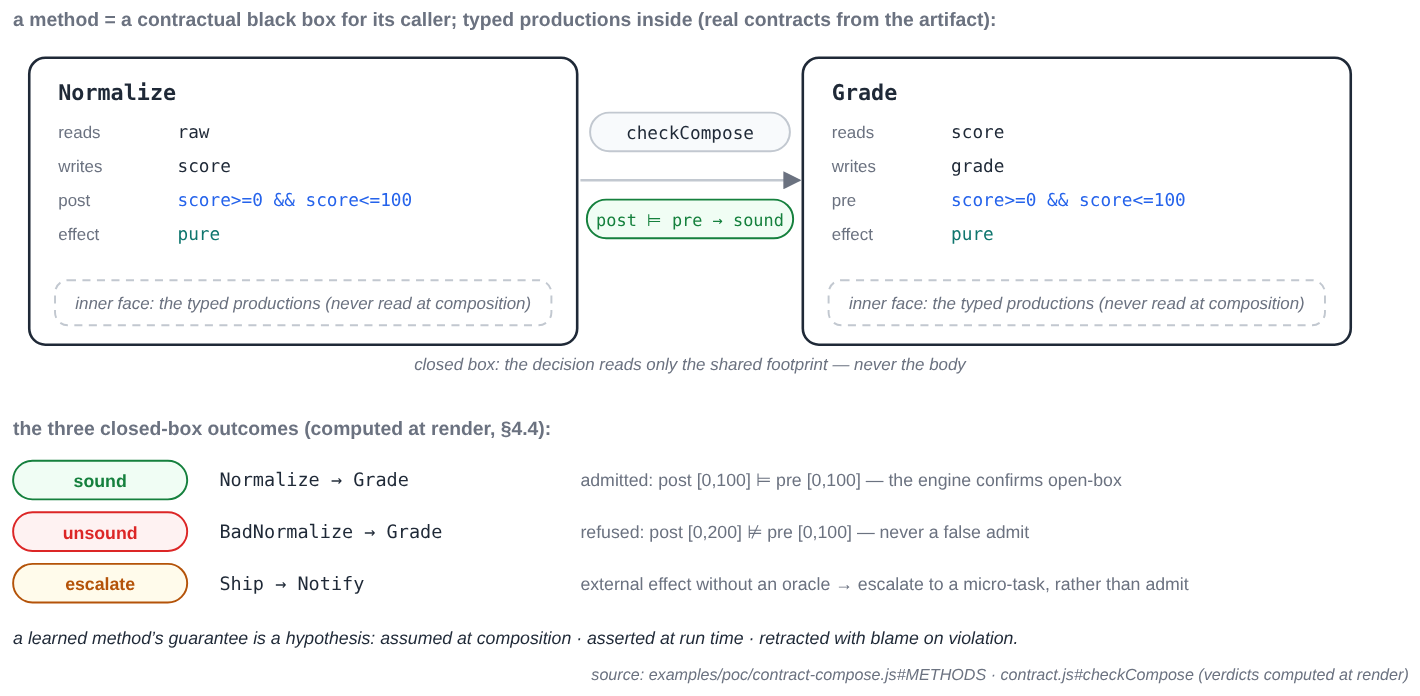
\includegraphics[width=\linewidth]{../figures/png/f1-method-contract.en.png}
\caption*{\small Figure F1 — the two-faced method: to its caller, a contractual black box (read/write footprints, pre/post, effect tag — the artifact's real contracts); inside, the typed productions, never read at composition. Between two methods, the closed-box \texttt{checkCompose} decision has three outcomes — sound / unsound / escalate —, computed as the figure is rendered (§4.4).}
\end{figure}

\subsection*{2.3 The pipeline and the K1 floor}

The third question remains: in what pipeline does this method live, and with what safety net when it is missing? The pipeline, end to end: a human formulation is typed into a goal; a method is selected and composed on its contracts; cases flow through it; traces distil into new typed methods (anti-unification [Plotkin 1970], MDL-gated as in DreamCoder/Stitch [Ellis et al. 2021; Bowers et al. 2023]); and drift retracts what it invalidates. The \emph{admission} step of this pipeline — under what conditions a unit learned from a noisy LLM episode may enter the library — is the subject of the companion article [Braun 2026b], which provides the localized-attribution admission gate (slot restriction, lattice edge, surface alias) that the loop described here assumes upstream.

The universal fallback is the \textbf{micro-task floor}: anything that does not reduce to a cached typed method reduces to a micro-task a small model does easily. So a \emph{missing} contract costs a cheap model call (a graceful cost gradient), and a \emph{wrong} contract is caught by the runtime assert — the two failure modes degrade cost and trigger un-learning respectively, never silent error.

\medskip\hrule\medskip

\section*{3. Implementation}

All mechanisms are realized on an existing rule-driven, JTMS-coherent typed-fact graph engine with declarative concepts and forward-chaining stabilization, with no changes to its core beyond one additive, backward-compatible query option. The typed memo key is the engine's canonicalization digest; the defeasible-contract checker (compose-time entailment over abstract domains, a runtime post-assertion, and three soundness gates) and the structural-transfer transform (relativize-on-store / bind-on-replay) are host libraries over the engine. A case executor that runs validated methods durably at scale is a known engineering artifact (a workflow net [van der Aalst 1998] over a durable store, in the lineage of AWS Step Functions Distributed Map [AWS 2022], Prefect's content cache, and DBOS [Skiadopoulos et al. 2021]); our \textbf{belief view} — the typed belief graph maintained by the JTMS, as opposed to that durable execution layer — sits above it.

The defeasible lifecycle — \textbf{assume → assert → verify → retract → specialize} — is the whole mechanism, mapping one-to-one onto the engine functions it calls:

\begin{small}\begin{verbatim}
select(goal):                                # ASSUME (compose time)
    M ← library.match(goal.typed_facts)      #   typed key; a miss falls to the micro-task floor
    assume M.contract                        #   checkCompose: post ⊨ pre — escalate
                                             #   rather than admit: never a false-admit

apply(M, case):                              # ASSERT + VERIFY (run time)
    key ← digest(case.typed_premise)         #   K1 canonical key
    if memo.has(key): return memo[key]       #   amortize a recurrent typed case
    out ← run(M, case)                       #   else derive (model call / sub-graph)
    if not assertPost(M.contract, out):      #   post holds? + G1 frame + G2 effect
        quarantine(case); blame(M.contract)  #   never commit a bad output
        return
    memo[key] ← out; return out

on ingest(fact):                             # RETRACT + SPECIALIZE (drift)
    for e in memo s.t. e depends on fact:    #   JTMS: re-assert each affected post
        if not satisfies(e.contract.post, e.facts ∪ {fact}):
            retract(e); blame(e.contract)    #   un-learn: evict + assign blame
    library.revise(blame): pre ← specialize(pre)
                                             #   reviseOnBlame (CEGIS, counterexample-guided):
                                             #   narrow the pre, do not delete
\end{verbatim}\end{small}

The verify-and-retract suffix is the only part absent from a similarity memory, and it is exactly the part the experiments isolate.

\begin{figure}[htbp]\centering
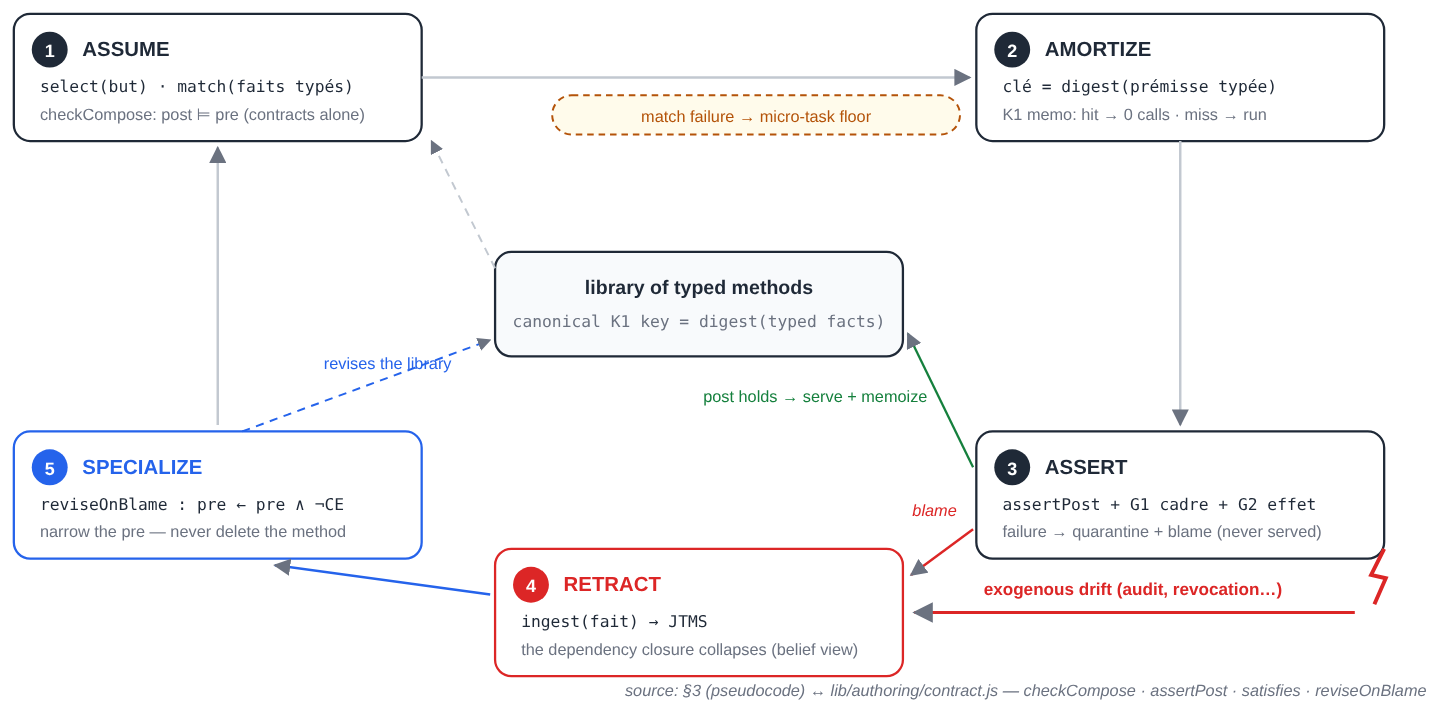
\includegraphics[width=\linewidth]{../figures/png/f2-defeasible-loop.en.png}
\caption*{\small Figure F2 — the defeasible lifecycle, in one-to-one correspondence with the engine functions it calls: assume (\texttt{checkCompose}), amortize (the canonical K1 key and its memo), assert (\texttt{assertPost} plus the frame and effect guards), retract (the JTMS, when exogenous drift fells a premise), specialize (\texttt{reviseOnBlame}). A selection miss falls back to the micro-task floor.}
\end{figure}

\medskip\hrule\medskip

\section*{4. Experiments}

The evaluation path: the shared setup (§4.1), then the decisive defeasance-on-drift test (E2, §4.2), sound amortization and transfer (E1, §4.3), composition soundness (E3, §4.4), the K1-coverage ceiling (P4, §4.5), scale (E5, §4.6), the head-to-head against named systems (E6, §4.7), composition under drift (E7, §4.8) and library revision (E8, §4.9). Each experiment opens on the §1 promise it checks.

\subsection*{4.1 Setup}

Experiments use the real engine's mechanisms, at two levels of fidelity that we state explicitly. E1 and E3 \textbf{instantiate the full engine} (\texttt{new Graph(...)} + stabilization + JTMS): E1 mounts structural methods and transfers them via the engine's relativize/bind; E3 composes real concepts and compares the box-closed \texttt{checkCompose} verdict to the engine's actual stabilization outcome. E2, P4, and E5 \textbf{isolate the relevant engine functions} — the canonicalization key (\texttt{digest}), the contract re-assertion (\texttt{satisfies}), the canonicalization barrier (\texttt{canonValue}) — driving them from a harness rather than the full stabilization loop, so that the \emph{mechanism} (typed key, defeasance, coverage) is measured without conflating it with the engine's scheduler. So "on the real engine" means the real functions throughout, and the full reactive loop for E1/E3; we do not claim E2 exercises the engine's native \texttt{\_revs}/JTMS retraction (it re-implements that retraction over the same real predicate). The model runs either as a \textbf{deterministic stub} (a perfect oracle of the \emph{current} rule given only what each arm's prompt reveals — so all staleness and cost come from each arm's mechanism, not model error) or as a \textbf{live} local model (Qwen3.6-27B (Q2\_K\_XL, MTP)). A shared prompt builder makes per-call context comparable across arms. Every comparative run is gated by a \textbf{harness self-test}: under the stub the naive arm must be perfectly correct, else the instrumentation is broken and the run aborts. All stub results are deterministic across re-runs. Seven arms share one interface:

\begin{itemize}
\item \textbf{Naive} — re-derive each record; \textbf{Long-context} — re-derive with all history in the prompt; \textbf{RAG} — reuse nearest by surface key: the obvious baselines;
\item \textbf{CBR} — reuse on the typed key, no re-validation;
\item \textbf{Skill} — a Voyager-style prose skill re-applied by the model;
\item \textbf{Invalidating} — the FAIR baseline: the typed-key cache plus a coarse hand-coded class-callback that drops a whole audited class on the audit event — an invalidation hook, but no typed contract;
\item \textbf{Struct} — the typed library with the defeasible contract: it re-asserts the post per entry, evicting only what is violated.
\end{itemize}

The Invalidating arm exists specifically to separate "has an invalidation mechanism" from "has a \emph{typed defeasible contract}."

\subsection*{4.2 E2 — defeasance on drift (the decisive test)}

A typed approval domain (N = 80, two audited classes; the live run uses N = 48, one audited class) with an \emph{external} mid-stream premise-invalidation: a compliance audit marks a class non-compliant, flipping its previously-approved cases to reject. The audit is \textbf{not a record field} — it is exogenous — so a recall-only cache retrieves the same unchanged record and serves its cached pre-audit answer. Here are the stub results:

\begin{center}\small\begin{adjustbox}{max width=\linewidth}\begin{tabular}{lllll}\toprule
arm & calls & overall acc & \textbf{drift acc} & max per-call ctx \\ \midrule
\textbf{Struct} (typed contract) & \textbf{26} & \textbf{1.00} & \textbf{1.00} & \textbf{290} \\
Invalidating (hook, no contract) & 28 & 1.00 & 1.00 & 290 \\
Naive & 80 & 1.00 & 1.00 & 290 \\
Long-context & 80 & 1.00 & 1.00 & 2062 \\
RAG & 48 & 0.95 & 0.00 & 290 \\
CBR (typed key, no re-validation) & 24 & 0.95 & 0.00 & 290 \\
Skill (prose) & 80 & 0.95 & 0.00 & 297 \\
\bottomrule\end{tabular}\end{adjustbox}\end{center}

The reading is three-fold. \textbf{Recall-only memories (RAG / CBR / Skill) serve stale} — recall alone cannot recover, because the audit never enters their reuse path. \textbf{Recovery requires an invalidation mechanism}, and \emph{both} the Invalidating cache and Struct have one, so both reach drift-acc 1.00. What the \textbf{typed defeasible contract adds over the hand-coded class-callback} comes down to three properties:

\begin{itemize}
\item \textbf{selectivity} — Struct re-asserts the post per entry (\texttt{satisfies}) and evicts only the 2 \emph{violated} (approve) classes, where the callback coarsely drops whole classes (4 entries) and pays the extra re-derivations (26 vs 28 calls);
\item \textbf{generality} — the same \texttt{assertPost} is premise-agnostic by construction (the experiments exercise one premise type, a compliance-flag flip), whereas the callback is per-event hand-coded;
\item \textbf{composition-safety} (§4.4). The
\end{itemize}
live run (Qwen3.6-27B (Q2\_K\_XL, MTP), N = 48) reproduces this exactly: RAG/CBR/Skill drift-acc 0.00; Invalidating 14 calls / drift 1.00; Struct 13 calls / 2.6 s / drift 1.00 / ctx 278 vs Long-context 1304 — recall-only stale, both invalidating arms recover, Struct selective.

\begin{figure}[htbp]\centering
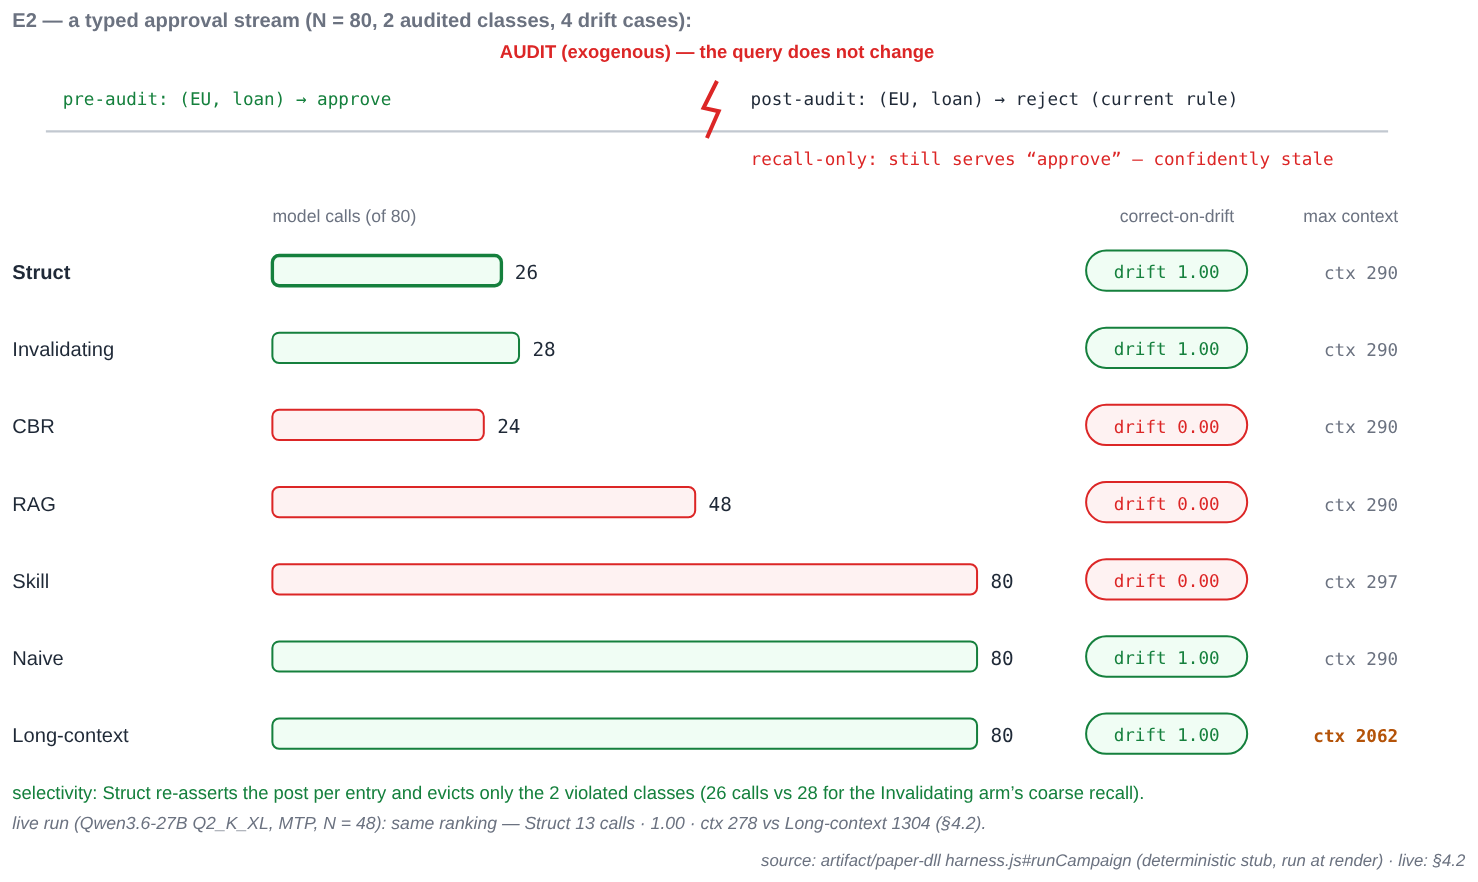
\includegraphics[width=\linewidth]{../figures/png/f3-e2-drift.en.png}
\caption*{\small Figure F3 — E2: the exogenous audit flips a class mid-stream without changing the query. Recall-only memories (red) serve stale; invalidation-equipped arms (green) recover; the typed contract recovers selectively (26 calls, 2 evictions — only the violated classes). Bars, verdicts and counts are recomputed at render time from the artifact's deterministic harness.}
\end{figure}

So E2's defensible claim is not "only Struct recovers" but "recall-only memory cannot un-learn, and a \emph{declarative typed contract} provides the recovery selectively, generally, and composition-safely."

\subsection*{4.3 E1 — amortization and structural transfer}

E2 showed recovery on drift; §1's other promise — reuse that amortizes \emph{without replaying wrong} — is checked here. The bench: a structural-decomposition domain (a method that \emph{creates} a sub-graph with object ids), on the \textbf{full engine}. The split: train, \textbf{held-out related} (same typed transitions, fresh id-spaces), and \textbf{held-out novel}. This is an existence-and-soundness check on a small set (2 held-out related, 1 novel), not a population rate: with the relativize/bind transform, \emph{all} held-out related instances transfer at 0 calls and \textbf{sound}, the novel transition pays (no false replay), and totals are 3 calls vs the no-cache baseline's 5. The no-transform ablation (a flat content cache) "hits" the related instances but replays the \emph{wrong id-space} — \textbf{unsound}.

The point is qualitative and is the most interesting finding in the paper: a call-count-only metric ranks the flat cache equal to the transform (both elide), so \textbf{only the soundness check distinguishes sound reuse from a wrong-id-space replay}. (Scaling this to a transfer \emph{rate} over many methods is future work; §6.)

\subsection*{4.4 E3 — composition soundness}

Third promise of §1: composing without opening the box. Composing method pairs purely on their typed contracts (box closed) and comparing to the open-the-box engine outcome (on the \textbf{full engine}), the box-closed decision \textbf{matches reality on every evaluated pair, with no false-admits} — the checker never false-accepts; under-determined or out-of-fragment pairs \emph{escalate} (to a micro-task) rather than admit. This is demonstrated on a small, hand-constructed set (3 composition pairs spanning sound / unsound / escalate; a 4th adds the oracle case), so it is an existence demonstration of soundness, not a population false-admit \emph{rate}. Each of three gates is shown load-bearing on a dedicated example: removing frame-completeness misses an undeclared write; removing the effect-tag gate silently admits an unverified external effect; removing footprint-cycle detection admits a coupled-retractable cycle. The decision reads only the shared footprint, never the body. (A larger, non-hand-picked method corpus is future work; §6.) We note the checker itself — per-key abstract-domain entailment, sound-but-incomplete, escalate-on-doubt — is the most developed formal artifact and is, if anything, under-evaluated here.

\subsection*{4.5 P4 — the K1-coverage ceiling}

There remains §1's K1 constraint: what does it actually cost? On a mixed workload (fraction \emph{p} fully typed; the rest carrying a prose component that overrides the typed rule), with K1-membership decided by the \textbf{real} canonicalization barrier, amortization is a \textbf{gradient in coverage} (approval: 0 → 19 → 44 → 69 → 94\% elided at p = 0/.25/.5/.75/1; triage: 0 → 22 → 47 → 72 → 97\%). Struct's accuracy is \textbf{1.00 at every coverage} — the non-typed fraction is a micro-task \emph{cost}, never a soundness \emph{cliff}. A greedy variant that memoizes prose-bearing records on their typed key drops to an accuracy equal to the clean fraction: \textbf{amortizing beyond the canonicalizable fraction is unsound}, so the K1 ceiling is a \emph{soundness boundary}, not a missed optimization. The result holds on both domains and is deterministic. We are explicit that this is a \textbf{constructed illustration}, not a measurement of a real workload: we \emph{set} the typed fraction \emph{p}, and the prose-bearing records are defined to override the typed rule, so "amortizing past K1 is unsound" follows by construction rather than by surprise. What it establishes is the \emph{shape} (amortization is proportional to coverage, not a constant win) and that soundness is preserved at every level; the canonicalizable fraction of a real corpus is domain-dependent and not measured here (§6).

\begin{figure}[htbp]\centering
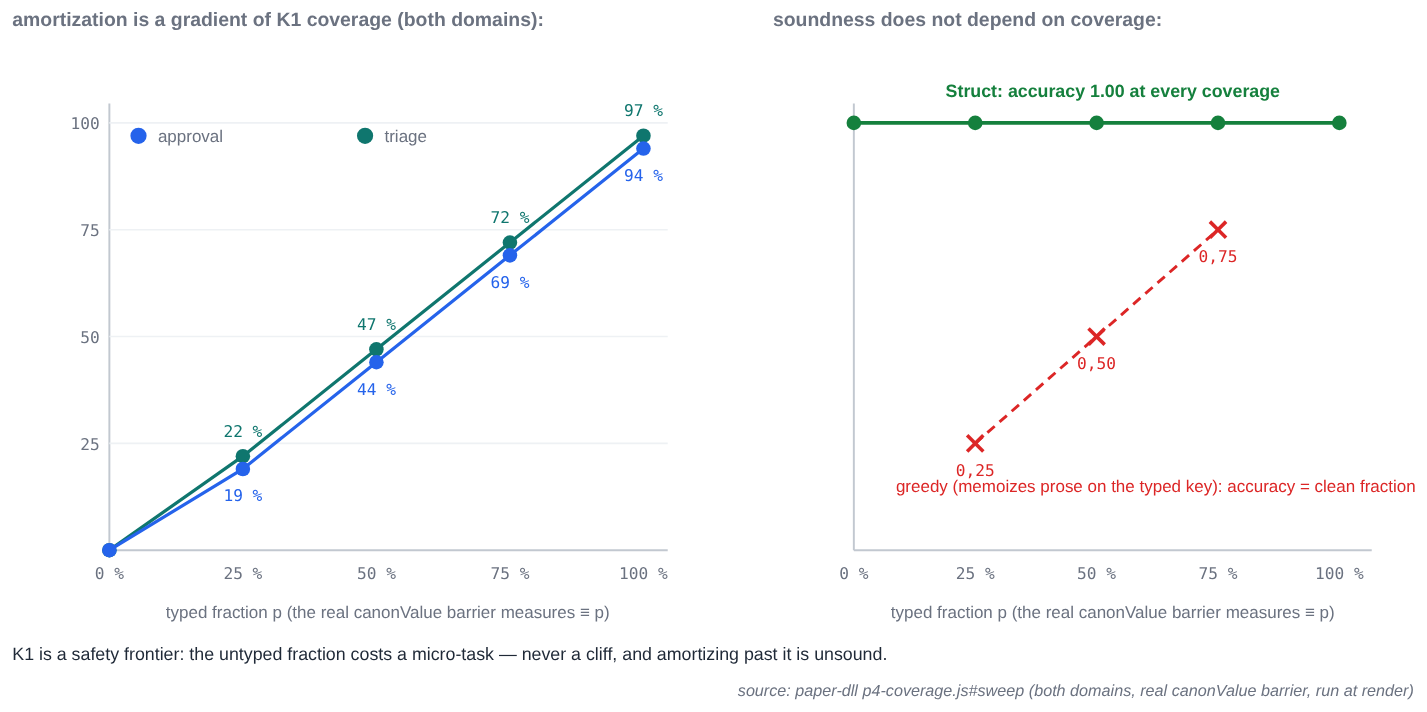
\includegraphics[width=\linewidth]{../figures/png/f6-p4-k1.en.png}
\caption*{\small Figure F6 — P4: amortization is a gradient of K1 coverage (left, both domains); soundness does not depend on it (right: 1.00 at every coverage, while the greedy negative control drops to the clean fraction). K1 is a safety frontier, not a missed optimization.}
\end{figure}

\subsection*{4.6 E5 — scale and per-mechanism cost}

A bookkeeping-cost check, not a claim about scaling the hard part — a growing library of \emph{distinct} methods, left to future work (end of section): over a 200-class typed space with one mid-stream audit, as the stream length N grows 1 320 → 20 320 (the \emph{class set} is fixed; no new methods, no model):

\begin{center}\small\begin{adjustbox}{max width=\linewidth}\begin{tabular}{llllll}\toprule
N & Struct calls & calls / N & Naive calls & library (memo) & evicted on drift \\ \midrule
1 320 & 202 & 0.153 & 1 320 & 200 & 2 \\
5 320 & 202 & 0.038 & 5 320 & 200 & 2 \\
20 320 & 202 & 0.010 & 20 320 & 200 & 2 \\
\bottomrule\end{tabular}\end{adjustbox}\end{center}

Struct's call count stays \textbf{constant} (the bounded number of distinct classes plus the drift re-derivations), so the per-record call rate falls toward zero while Naive stays at one; the library size is bounded by the class count (trivially — it is a map keyed on a bounded class set); and a drift event \textbf{retracts only the invalidated classes} (O(invalidated): 2 evictions over a 200-entry library, not O(library)). Per-operation costs are small: canonicalization is low-single-digit µs/call (environment-dependent), and a single drift's eviction pass is ≈ 0.5 ms over the whole library. What E5 establishes is narrow: the typed bookkeeping (key, memo, selective eviction) does not become the bottleneck as the stream grows. This experiment does \textbf{not}, however, test scaling in the dimension that matters — a growing library of \emph{distinct} methods, a real corpus, or a live model across all arms — which we leave to future work (§6).

\subsection*{4.7 E6 — head-to-head against named agent-memory systems}

The §4.1 baselines are generic (RAG / CBR / Skill). The systems a reviewer compares against are the \emph{named} ones: \textbf{MemGPT/Letta} (tiered virtual context with self-editing memory) [Packer et al. 2023], \textbf{Reflexion} (an episodic verbal-reflection retry driven by a failure signal) [Shinn et al. 2023], and \textbf{GraphRAG} (an offline knowledge-graph index with LLM community summaries) [Edge et al. 2024]. We add a faithful minimal re-implementation of each behind the same interface, each in its \emph{fairest} configuration, with a paired ablation that turns its distinctive mechanism off (the negative control). The bench is a deterministic stub: N = 78, two audited classes, six drift cases:

\begin{center}\small\begin{adjustbox}{max width=\linewidth}\begin{tabular}{lllll}\toprule
arm & model calls & acc & drift-acc & max ctx \\ \midrule
Naive & 78 & 1.00 & 1.00 & 290 \\
\textbf{MemGPT} (audit paged into core) & 23 & 1.00 & 1.00 & 320 \\
MemGPT − paging (ablation) & 18 & 0.92 & 0.00 & 258 \\
\textbf{Reflexion} (delayed failure signal) & 82 & 1.00 & 1.00 & 332 \\
Reflexion − signal (ablation) & 78 & 0.92 & 0.00 & 258 \\
\textbf{GraphRAG} (offline index) & 87 & 0.92 & 0.00 & 336 \\
GraphRAG + re-index (ablation) & 89 & 1.00 & 1.00 & 336 \\
\textbf{Struct} & \textbf{20} & \textbf{1.00} & \textbf{1.00} & \textbf{290} \\
\bottomrule\end{tabular}\end{adjustbox}\end{center}

\begin{figure}[htbp]\centering
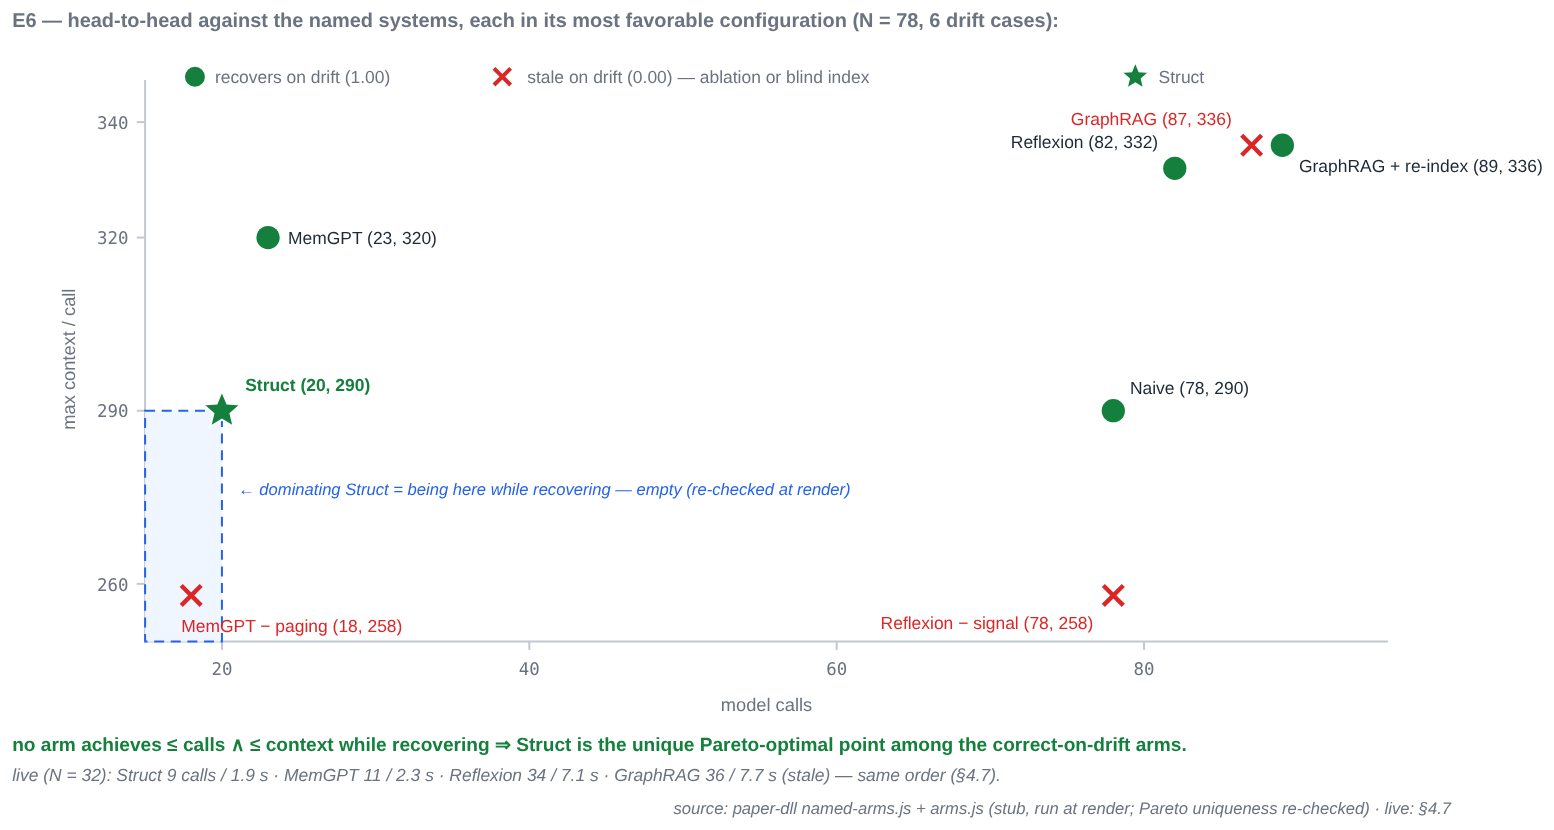
\includegraphics[width=\linewidth]{../figures/png/f4-e6-pareto.en.png}
\caption*{\small Figure F4 — E6 on the (calls × per-call context) plane: green = recovers on drift, red = stale. The dashed region — ≤ calls and ≤ context than Struct — is empty among the recovering arms: Struct is the unique Pareto-optimal point, uniqueness re-checked at render time.}
\end{figure}

The honest reading is \emph{not} "only Struct recovers": given its fairest shot, each named system \textbf{can} recover correctness on drift (MemGPT and Reflexion reach drift-acc 1.00; GraphRAG does once it re-indexes).

The claim is that Struct recovers at the lowest cost on all three axes \emph{at once} — it is the only arm that recovers on drift while remaining undominated (no arm beats-or-ties it on calls AND per-call context while also recovering; the cheaper arms sit on the cost frontier but fail on drift). Each named system pays a different mechanism-specific tax:

\begin{itemize}
\item \textbf{MemGPT} recovers only once the exogenous audit is surfaced and self-edited into core memory (a model turn); the recovery is then \emph{coarse} — a whole-(region,kind)-class flag that re-decides even the unaffected low-score members (over-eviction, +calls) — and a core-memory block rides in every prompt (+context).
\item \textbf{Reflexion} has \emph{no content-addressed memo}, so it issues a model call on \textbf{every} record (calls ≈ N — the decisive gap), and recovers only \emph{reactively}, after observing a failure, via a stored prose reflection (a recovery lag + prepended context).
\item \textbf{GraphRAG}'s offline index is blind to the silent audit, so it is stale by default; recovery requires a \textbf{batch re-summarization} of affected communities (coarse, per-community, off-band), never a per-entry defeater. (GraphRAG is off-design for point decisions — its strength is global sensemaking; this stress-tests the named graph-retrieval system on the defeasance axis.)
\end{itemize}

The named systems were not designed to amortize recurrent typed point-decisions; this workload stresses them off-design, so the "tax" is the cost of a mismatched tool, not inferiority at their own task. The ablations confirm each mechanism is load-bearing (turn it off → drift-acc 0.00). Measured \emph{in isolation} (calls on the drifting stream minus calls on a no-drift twin), Struct's recovery tax is the re-derivation of only the \textbf{violated} cached entries (2; selective), and the contract re-assertion itself is in-engine — \textbf{zero} model calls — strictly below each named system's. A live run (Qwen3.6-27B (Q2\_K\_XL, MTP), N = 32) reproduces the ordering: Struct \textbf{9} calls / 1.9 s, MemGPT 11 / 2.3 s, Reflexion 34 / 7.1 s, GraphRAG 36 / 7.7 s (stale); Struct is the unique Pareto-optimal point among the drift-correct arms live too. These are minimal faithful re-implementations of each mechanism, not the full systems (§6).

\subsection*{4.8 E7 — composition under drift}

E6 measures a \emph{single} method. The differentiator of a \emph{library} is composition: when an upstream method's premise falls, does the recovery propagate through the chain? We extend the workload to a two-link chain — \texttt{decide → disburse}, where \texttt{disbursement = disbursed iff decision == approve} (link 2 reads link 1's outcome fact) — and re-run the head-to-head, scoring \textbf{both} links. The same exogenous audit now cascades: an audited high-score case must flip \texttt{decision} approve→reject \textbf{and} \texttt{disbursement} disbursed→held. Two regimes are run: the deterministic stub (N = 78, two audited classes) and a live run (Qwen3.6-27B (Q2\_K\_XL, MTP), N = 48):

\begin{center}\small\begin{adjustbox}{max width=\linewidth}\begin{tabular}{llll}\toprule
arm & calls (stub / live) & drift-acc link 1 & drift-acc link 2 \\ \midrule
Naive & 156 / 96 & 1.00 & 1.00 \\
CBR (= Struct − contract) & 36 / 24 & \textbf{0.00} & \textbf{0.00} \\
MemGPT (fairest) & 45 / 41 & 1.00 & 1.00 \\
Reflexion (fairest) & 160 / 108 & 1.00 & 1.00 \\
GraphRAG + re-index & 178 / 116 & 1.00 & 1.00 \\
\textbf{Struct} & \textbf{38 / 26} & \textbf{1.00} & \textbf{1.00} \\
Struct (full engine) & 38 / 27 & 1.00 & 1.00 \\
\bottomrule\end{tabular}\end{adjustbox}\end{center}

Three things are measured. (i) \textbf{Staleness compounds.} Every recall-only or blind arm (CBR, and each named system's ablation) is wrong at link 1 \emph{and} link 2: a stale upstream answer poisons the downstream that reads it. Drift correctness is measured on the deterministic oracle; the live run confirms the CALL/WALL ordering (the live model is imperfect at small N, so we do not read per-record drift off it). (ii) \textbf{The recovery tax multiplies down the chain.} Reflexion, having no memo, pays a call per record \emph{per link} (calls ≈ 2N); GraphRAG re-indexes affected communities at \emph{each} link; MemGPT pays paging + coarse re-decode + a larger context at \emph{both} links. (iii) \textbf{Struct's cascade is selective.} A fallen premise un-casts the upstream belief and the change propagates to the downstream — recovering both links while re-deriving \emph{only} the violated upstream entry (the downstream re-derivation is elided because its cache key is disburse's true read-set \texttt{\{kind, region, decision\}}). Struct is the unique Pareto-optimal point among the drift-correct arms on (calls × drift-acc link 1 × drift-acc link 2 × per-call context), stub and live; the full-engine realization (four ensure-gated concepts over the derivation cache) reproduces it (38 = 38 stub; 26 ≈ 27 live, within model nondeterminism).

\begin{figure}[htbp]\centering
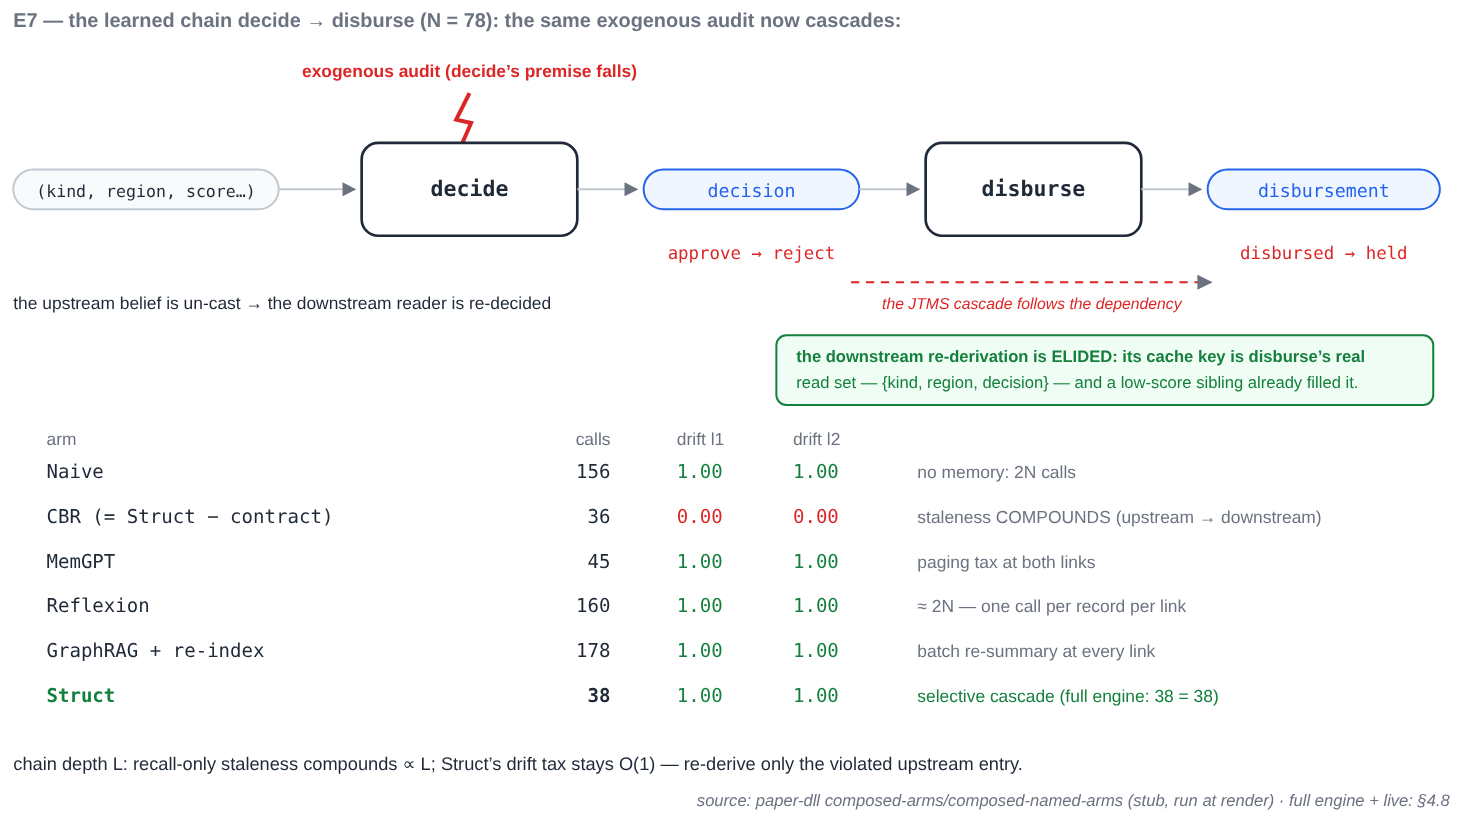
\includegraphics[width=\linewidth]{../figures/png/f5-e7-cascade.en.png}
\caption*{\small Figure F5 — E7: drift through the learned chain decide → disburse. The upstream premise falls; the JTMS cascade retracts the decision and the disbursement that reads it; only the violated upstream entry is re-derived — the downstream re-derivation is elided by its read-set cache key, already filled by a sibling. Table recomputed at render time.}
\end{figure}

This is the capability the named surface memories structurally lack: a belief that depends on a premise which just fell, un-learned \emph{across composition}.

\textbf{The wedge widens with chain depth.} Generalising the chain to L links (each positive iff the previous is), the staleness and the cost both scale while Struct's recovery does not: a recall-only cache's \emph{compounding depth} (links wrong on a drifted class) is exactly L; Naive and Reflexion pay O(L·N) calls; but Struct's recovery \textbf{drift-tax is O(1) in L} — the cascade re-derives only the violated upstream entry, every downstream re-derivation reusing a sibling's read-set entry. So the deeper the learned method chain, the larger Struct's advantage on the correctness gap (compounding ∝ L) and on recovery efficiency (O(1) vs an O(L) coarse rebuild). (O(1) recovery holds when each downstream re-derivation collapses onto a cache key a sibling already filled — true here: the negative branch is shared and low-score siblings pre-fill it; under high downstream fan-out the recovery tax grows toward O(L). The compounding ∝ L follows by construction from defining link \emph{i} as a function of link \emph{i}−1, and is \textbf{measured on the deterministic stub} — the live L-sweep is noise-confounded, §6.)

\textbf{On the real durable executor.} The above is the belief view (the rule-driven graph + JTMS retraction). The same chain compiled to a workflow net and run as a token-flow over a content-addressed, crash-resumable checkpoint store reproduces the result on the \emph{execution} layer: the chain amortizes and the drift cascades through both links (Struct-on-executor 24 calls, drift 1.00/1.00; the premise-less key and a flat composed cache both compound), the warm composed library \textbf{replays across a process restart at zero model calls}, and a chain cut mid-flight \textbf{resumes with no work lost or duplicated}. Rebuilding only the affected link rather than the whole chain places this in the lineage of self-adjusting computation [Acar, Blelloch \& Harper 2002] and minimal-rebuild build systems [Mokhov, Mitchell \& Peyton Jones 2018]. Belief-view defeasance and durable execution are complementary: the contract retracts the belief; the executor makes the recomputation durable and selective.

\subsection*{4.9 E8 — library revision under recurrent drift}

E2/E6/E7 measure the \emph{retract → re-derive} path: a violated post evicts the cached belief, which is then re-derived. The loop's other half — \emph{revise}: specialize the method's precondition on blame, so the library is improved, not merely re-evaluated — is evaluated here. We run K = 5 recurrent-drift episodes (the same classes recur each episode after an over-general precondition is exposed) and compare evict-only against revision via the engine's \texttt{reviseOnBlame}:

\begin{center}\small\begin{adjustbox}{max width=\linewidth}\begin{tabular}{lll}\toprule
over K=5 episodes & Evict-only & Revise (\texttt{reviseOnBlame}) \\ \midrule
blames (per episode → cumulative) & 1,1,1,1,1 → 5 & 1,0,0,0,0 → 1 \\
re-derivations (model calls) & 4,1,1,1,1 → 8 & 4,1,0,0,0 → 5 \\
false-admit rate & 0.25 every episode & 0.25 → 0.00 after e1 \\
\bottomrule\end{tabular}\end{adjustbox}\end{center}

Evict-only keeps the over-general rule, so it re-admits, re-blames, and re-derives the same stale class \emph{every} episode (cost ∝ K). Revision specializes the precondition once — narrowing it with the counterexample's discriminating atom — and then flatlines: no further blames, false-admit → 0. The revision is \emph{surgical}: the specialized precondition excludes the failing class while still admitting its sibling (it narrows, it does not delete the method). The effect holds for two premise kinds — a categorical compliance flip (\texttt{\$compliant != false}) and a numeric gate (\texttt{\$score != 680}). \textbf{Honest limit:} \texttt{reviseOnBlame} specializes by counterexample point-exclusion, not bound-tightening; a numeric drift spanning D distinct values converges in D one-time blames (bounded, per-value) rather than a single bound move — still categorically better than evict-only's per-episode recurrence.

\begin{figure}[htbp]\centering
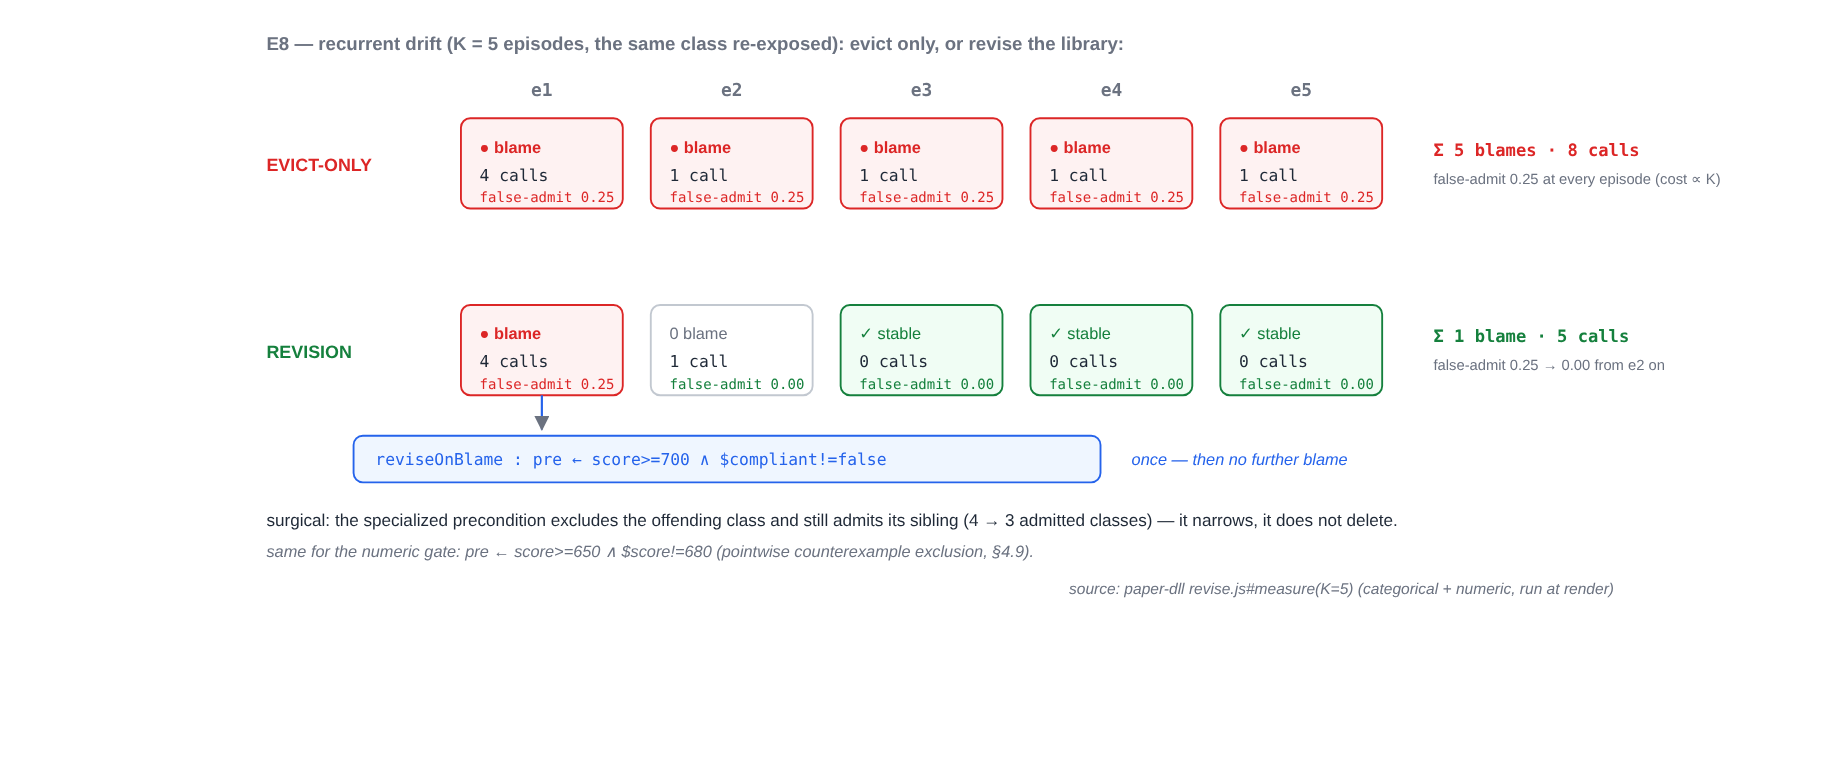
\includegraphics[width=\linewidth]{../figures/png/f7-e8-revision.en.png}
\caption*{\small Figure F7 — E8: under recurrent drift (K = 5), evict-only re-blames and re-pays the same class every episode; revision specializes the precondition once (\texttt{reviseOnBlame}, with the real discriminating atom) and then flatlines — surgical: the sibling stays admitted.}
\end{figure}

This is the step that distinguishes the contract from cache invalidation (§5): blame feeds \emph{library revision}, not just value recomputation.

\medskip\hrule\medskip

\section*{5. Related Work}

The neighborhoods are visited from the most obvious to the closest: recall memories (retrieval/case, then the named agent memories, then long context), learned libraries, contracts, the composition frames, theory revision — the nearest neighbor —, truth maintenance, and finally the plumbing (durable execution, view maintenance) over which we claim nothing.

\textbf{Retrieval and case memory.} RAG [Lewis et al. 2020] and CBR [Aamodt \& Plaza 1994] recall by surface/embedding similarity and reuse-or-adapt; they cannot represent a \emph{premise becoming invalid}, so an exogenous change that leaves the query unchanged leaves the cached answer retrievable and stale (E2). Skill libraries such as Voyager [Wang et al. 2023] store reusable \emph{prose} skills with no typed, defeasible premise, so a stale skill stays applicable and must be re-applied by the model — cost without correctness (our Skill arm). Our typed premise lives in the belief, so when it falls the derivation retracts (JTMS) and the library narrows the method.

\textbf{LLM agent memory.} Recent agent-memory systems manage \emph{what to keep and recall} far more cleverly than vanilla RAG — MemGPT/Letta's tiered virtual context [Packer et al. 2023], Reflexion's episodic verbal-reflection buffer [Shinn et al. 2023], and graph-structured retrieval such as GraphRAG [Edge et al. 2024]. But they recall and reuse by relevance, recency, or similarity and, to our knowledge, none represent a \emph{typed premise whose falsification retracts a prior reuse}. These systems are complementary rather than competing: a defeasible contract could sit beneath any of them as the retraction layer. We run this head-to-head in \textbf{§4.7 (E6)}: each, given its fairest shot, can recover on drift, but only the defeasible contract does so at the lowest cost on (calls × correctness × context) simultaneously — the others pay a paging / per-record / batch-re-index tax.

\textbf{Long context.} Carrying full history per call is correct but O(N) in per-call context (E2: 2062 vs 290) with no structural reuse.

\textbf{Library learning / EBL.} DreamCoder [Ellis et al. 2021] and Stitch [Bowers et al. 2023] grow a library by abstraction (anti-unification / MDL [Plotkin 1970]); EBG [Mitchell, Keller \& Kedar-Cabelli 1986] specializes from a single proof. These learn \emph{what} to reuse but attach no defeasible runtime contract that un-learns on drift; we add that contract and its blame-driven revision.

\textbf{The companion article: admission of learned units.} The present article assumes that what enters the library was soundly admitted from noisy LLM episodes. That admission problem — making candidate elimination tolerant to an LLM's incompetence noise through a localized-attribution gate, applied at the slot-restriction, \emph{isa}-edge and surface-alias grains — is treated and measured in [Braun 2026b]. The two articles share the engine, the typed-fact discipline and the recoverability semantics; this one carries the library's \emph{life} (amortize, compose, un-learn), that one its \emph{front door}.

\textbf{Contracts, blame, gradual verification.} Higher-order contracts with blame [Findler \& Felleisen 2002] and gradual/hybrid verification [Bader, Aldrich \& Tanter 2018] are the lineage of our assume/assert/retract-blame discipline; we apply it to \emph{learned} methods, routing blame into a library revision rather than an error.

\textbf{Composition: graph grammars, HTN, separation logic.} A method is a two-faced HRG non-terminal [Habel 1992; Drewes, Kreowski \& Habel 1997; Courcelle 1990] with HTN precondition-gated selection [Erol, Hendler \& Nau 1994]; recursive HTN plan-existence is undecidable [Erol, Hendler \& Nau 1996], so the grammar is kept decidable by a well-founded mount-rank while execution is explicitly fuel-bounded. Sound composition under shared state is the frame problem [McCarthy \& Hayes 1969], discharged by a separation-logic footprint discipline [O'Hearn, Reynolds \& Yang 2001; Reynolds 2002] over a finite typed alphabet (E3).

\textbf{Theory revision and belief revision (the nearest neighbor).} \texttt{reviseOnBlame} — specialize a learned precondition from a counterexample rather than delete the method — is, squarely, \textbf{theory revision / refinement} of a \emph{learned} rule base: EITHER [Ourston \& Mooney 1994] and FORTE [Richards \& Mooney 1995] revise Horn-clause theories on contradicting examples, exactly our blame→specialize step. At the logical level the contraction/ revision of a belief set on a new fact is \textbf{AGM belief revision} [Alchourrón, Gärdenfors \& Makinson 1985], and the runtime monitor sits in the \textbf{defeasible/non-monotonic reasoning} tradition [Reiter 1980]. We do not claim a new revision operator; our contribution relative to this line is operational — attaching the revision to a \emph{typed, composable, canonicalizable method library} with a runtime contract, so amortization, composition-checking, and un-learning share one representation. A reviewer from this community will rightly read the work as theory revision wrapped in a typed-contract, amortizing library; we agree, and position it as such.

\textbf{Truth maintenance.} The un-learn mechanism is a JTMS [Doyle 1979; de Kleer 1986]: a retracted premise cascades to its dependency closure, serving no wrong belief — the defeasance the baselines lack.

\textbf{Durable execution and workflow nets.} A case is an uncoloured 1-safe marking over a workflow net [van der Aalst 1998]; the durable executor that runs validated methods at scale is a known artifact [AWS 2022; Prefect; Skiadopoulos et al. 2021]. Rebuilding only the affected derivation rather than the whole chain is the spirit of self-adjusting computation [Acar, Blelloch \& Harper 2002] and minimal-rebuild build systems [Mokhov, Mitchell \& Peyton Jones 2018]. Our belief view sits atop such a layer; we do not reinvent the plumbing.

\textbf{Incremental view maintenance and cache invalidation.} DBSP [Budiu et al. 2023] / Materialize maintain \emph{values} incrementally, and production caches invalidate on source change — both are, in effect, the "invalidation hook" our fair baseline models, and we do not claim novelty over them for \emph{recovering} on drift. The difference we claim is narrow: our object is a typed, \emph{defeasible}, auditable belief whose invalidation is \textbf{derived from a declarative contract} (re-assert the post; blame; specialize the precondition), rather than a hand-specified view or a per-source invalidation rule — so it generalizes across premises and feeds library revision, not just value recomputation (measured in §4.9, E8).

\medskip\hrule\medskip

\section*{6. Threats to Validity}

Eight threats, from the most debated to the most structural: the stub, the parameterized K1 coverage, the strength of the generic baselines, the fidelity of the named re-implementations, the novelty positioning, scale and breadth, eventual soundness, and the single engine.

\textbf{Stub vs. live model.} The deterministic stub removes model error to isolate each arm's \emph{mechanism} — the very thing we claim about. It makes the comparison reproducible, and the \textbf{live} E2 run confirms the same ordering with a real model, where staleness is actually produced by the model following stale prose or a cache hit. The stub is not claimed to predict absolute live accuracy; running more arms live (E1/E3/P4 are engine-mechanism experiments and use the model as a call counter) is future work. Drift correctness is measured on the deterministic oracle; the live run confirms the CALL/WALL ordering (the live model is imperfect at small N, so we do not read per-record drift off it).

\textbf{K1-coverage is parameterized.} P4 \emph{sets} the typed fraction and \emph{measures} it via the real barrier; the non-circular claims are the \textbf{shape} (a gradient), the \textbf{universality of soundness} (1.0 at every coverage), and the \textbf{soundness boundary} (greedy amortization is unsound). The absolute canonicalizable fraction of any given production workload is domain-dependent and not claimed to be high everywhere.

\textbf{Baseline strength.} RAG/CBR/Skill are our implementations; the \textbf{Invalidating} baseline isolates "has an invalidation hook" from "has a typed contract," so the claim is precise: recall-only memory cannot recover, while a \emph{declarative typed contract} recovers selectively (post-violated only), generally (any premise), and composition-safely. A \emph{tuned} event-invalidating RAG/CBR is essentially the Invalidating arm and is expected to match Struct on drift-accuracy, differing only on selectivity/generality. The \textbf{named} agent-memory systems are evaluated directly in E6 (§4.7).

\textbf{Named-system fidelity (E6).} MemGPT, Reflexion, and GraphRAG are reproduced as \emph{minimal faithful arms} — each captures its distinctive mechanism (tiered self-editing memory / failure-driven verbal reflection / offline community-summary index) in its fairest configuration, but none is the full deployed system (no real LLM-driven memory edits, no learned reward model, no Leiden communities or embedding retrieval). Every simplification is \emph{charitable} — idealized audit surfacing, lossless summaries, exact retrieval — so each arm is an upper bound on its system's drift behavior, not a strawman; the load-bearing weakness we exhibit (coarse prose memory / no typed memo / blind offline index) is intrinsic to each design, not an artifact of the reduction. Symmetrically, our own STRUCT is \emph{not} a stub: a real-engine realization — concepts with ensure-gated JTMS retraction over the derivation cache — reproduces its measured corner both stub and live (9 calls on the live N = 32, matching the arm) and the warm library survives a restart at zero model calls, so E6 compares the named-system \emph{re-implementations} against the \emph{actual} engine, not stub-against-stub.

\textbf{Novelty / positioning.} No mechanism is new; the work is a \emph{composition} of JTMS, contracts-with-blame, library learning, and separation-logic footprints, and \texttt{reviseOnBlame} is theory revision (EITHER/FORTE). We position the contribution as the operational unification — typed amortizable library + composition-checking + un-learning in one representation — not as a new learning or revision algorithm.

\textbf{Scale and breadth.} The mechanism experiments (E1–E3, P4) use modest N (≤ 80 per E2 run) over two synthetic domains with known ground truth; E5 extends the \emph{deterministic} measurements to N ≈ 20 k and a 200-method library (showing amortization, bounded growth, and selective retraction hold with cheap per-op costs). The head-to-head against modern agent-memory systems (MemGPT/Letta, Reflexion, GraphRAG) is now E6 (§4.7), albeit with minimal faithful re-implementations; what remains future work is scale with a \emph{live} model and a \emph{real} corpus on a durable executor, and a comparison against the \textbf{deployed} systems rather than mechanism re-implementations.

\textbf{Soundness is eventual, not static.} Applicability of a learned method is undecidable in general (Rice), so the guarantee is eventual soundness via a load-bearing runtime monitor over a sound-but-incomplete compose-time gate. The monitor must run; its absence reintroduces false-admits, as E3's ablations show.

\textbf{Single engine / single author.} All results are on one implementation; independent reproduction on a different substrate would strengthen the structural claims.

\medskip\hrule\medskip

\section*{7. Conclusion}

Recall-only agent memory cannot un-learn; static libraries are sound but frozen. A learned library of typed methods with a \textbf{defeasible runtime contract} gets both: it amortizes and composes on typed structure, and when a premise drifts it \emph{retracts with blame and revises} — recovering correctness where retrieval, CBR, and skill libraries serve stale. Our experiments isolate this: recall alone cannot recover; an invalidation hook can; and a \emph{declarative typed contract} provides that recovery selectively, generally, and composition-safely, at bounded per-call context, on a real engine and confirmed on a live model — all under a canonicalizable fraction that is itself a soundness boundary. Every mechanism is prior art (JTMS, contracts-with-blame, theory revision, library learning, separation logic); the contribution is their composition into a single typed representation in which amortization, composition-checking, and un-learning coincide. It is, deliberately, an engineering synthesis with a testable emergent property — principled, selective un-learning — rather than a new algorithm; we think that property is worth naming and measuring.

\medskip\hrule\medskip

\section*{References}

\begin{itemize}
\item A. Aamodt, E. Plaza. \emph{Case-Based Reasoning: Foundational Issues, Methodological Variations, and System Approaches.} AI Communications 7(1):39–59, 1994.
\item U. A. Acar, G. E. Blelloch, R. Harper. \emph{Adaptive Functional Programming.} POPL 2002, pp. 247–259.
\item C. E. Alchourrón, P. Gärdenfors, D. Makinson. \emph{On the Logic of Theory Change: Partial Meet Contraction and Revision Functions.} Journal of Symbolic Logic 50(2):510–530, 1985.
\item AWS. \emph{Step Functions Distributed Map — A Serverless Solution for Large-Scale Parallel Data Processing.} AWS, 2022.
\item J. Bader, J. Aldrich, É. Tanter. \emph{Gradual Program Verification.} VMCAI 2018, LNCS 10747, pp. 25–46.
\item L. Bourtoule, V. Chandrasekaran, C. A. Choquette-Choo, H. Jia, A. Travers, B. Zhang, D. Lie, N. Papernot. \emph{Machine Unlearning.} IEEE Symposium on Security and Privacy 2021, pp. 141–159.
\item N. Braun. \emph{Sound online growth of a typed isa lattice from noisy LLM extraction, through candidate elimination made noise-tolerant by a localized-blame admission gate.} Preprint, 2026. [Braun 2026b — the companion admission-gate article]
\item M. Bowers, T. X. Olausson, L. Wong, G. Grand, J. B. Tenenbaum, K. Ellis, A. Solar-Lezama. \emph{Top-Down Synthesis for Library Learning.} POPL 2023; Proc. ACM Program. Lang. 7(POPL).
\item M. Budiu, T. Chajed, F. McSherry, L. Ryzhyk, V. Tannen. \emph{DBSP: Automatic Incremental View Maintenance for Rich Query Languages.} PVLDB 16(7):1601–1614, 2023.
\item B. Courcelle. \emph{The Monadic Second-Order Logic of Graphs I: Recognizable Sets of Finite Graphs.} Information and Computation 85(1):12–75, 1990.
\item J. de Kleer. \emph{An Assumption-based TMS.} Artificial Intelligence 28(2):127–162, 1986.
\item J. Doyle. \emph{A Truth Maintenance System.} Artificial Intelligence 12(3):231–272, 1979.
\item F. Drewes, H.-J. Kreowski, A. Habel. \emph{Hyperedge Replacement Graph Grammars.} In Handbook of Graph Grammars and Computing by Graph Transformation, Vol. 1 (G. Rozenberg, ed.), World Scientific, pp. 95–162, 1997.
\item D. Edge, H. Trinh, N. Cheng, J. Bradley, A. Chao, A. Mody, S. Truitt, J. Larson. \emph{From Local to Global: A Graph RAG Approach to Query-Focused Summarization.} arXiv:2404.16130, 2024.
\item K. Ellis, C. Wong, M. Nye, M. Sablé-Meyer, L. Morales, L. Hewitt, L. Cary, A. Solar-Lezama, J. B. Tenenbaum. \emph{DreamCoder: Bootstrapping Inductive Program Synthesis with Wake-Sleep Library Learning.} PLDI 2021.
\item K. Erol, J. Hendler, D. S. Nau. \emph{UMCP: A Sound and Complete Procedure for Hierarchical Task-Network Planning.} AIPS 1994.
\item K. Erol, J. Hendler, D. S. Nau. \emph{Complexity Results for HTN Planning.} Annals of Mathematics and Artificial Intelligence 18:69–93, 1996.
\item R. B. Findler, M. Felleisen. \emph{Contracts for Higher-Order Functions.} ICFP 2002, pp. 48–59.
\item A. Habel. \emph{Hyperedge Replacement: Grammars and Languages.} LNCS 643, Springer, 1992.
\item P. Lewis, E. Perez, A. Piktus, F. Petroni, V. Karpukhin, N. Goyal, H. Küttler, M. Lewis, W. Yih, T. Rocktäschel, S. Riedel, D. Kiela. \emph{Retrieval-Augmented Generation for Knowledge-Intensive NLP Tasks.} NeurIPS 2020.
\item J. McCarthy, P. J. Hayes. \emph{Some Philosophical Problems from the Standpoint of Artificial Intelligence.} Machine Intelligence 4, 1969.
\item T. M. Mitchell, R. M. Keller, S. T. Kedar-Cabelli. \emph{Explanation-Based Generalization: A Unifying View.} Machine Learning 1(1):47–80, 1986.
\item A. Mokhov, N. Mitchell, S. Peyton Jones. \emph{Build Systems à la Carte.} Proc. ACM Program. Lang. 2(ICFP), Art. 79, 2018.
\item P. W. O'Hearn, J. C. Reynolds, H. Yang. \emph{Local Reasoning about Programs that Alter Data Structures.} CSL 2001, LNCS 2142, pp. 1–19.
\item D. Ourston, R. J. Mooney. \emph{Theory Refinement Combining Analytical and Empirical Methods.} Artificial Intelligence 66(2):273–309, 1994.
\item C. Packer, S. Wooders, K. Lin, V. Fang, S. G. Patil, I. Stoica, J. E. Gonzalez. \emph{MemGPT: Towards LLMs as Operating Systems.} arXiv:2310.08560, 2023.
\item G. D. Plotkin. \emph{A Note on Inductive Generalization.} Machine Intelligence 5:153–163, 1970.
\item Prefect. \emph{Caching} (result/task caching by cache key). Prefect 3 documentation.
\item R. Reiter. \emph{A Logic for Default Reasoning.} Artificial Intelligence 13(1–2):81–132, 1980.
\item J. C. Reynolds. \emph{Separation Logic: A Logic for Shared Mutable Data Structures.} LICS 2002, pp. 55–74.
\item B. L. Richards, R. J. Mooney. \emph{Automated Refinement of First-Order Horn-Clause Domain Theories.} Machine Learning 19(2):95–131, 1995.
\item N. Shinn, F. Cassano, A. Gopinath, K. Narasimhan, S. Yao. \emph{Reflexion: Language Agents with Verbal Reinforcement Learning.} NeurIPS 2023.
\item A. Skiadopoulos, et al. \emph{DBOS: A DBMS-oriented Operating System.} PVLDB 15(1):21–30, 2021.
\item W. M. P. van der Aalst. \emph{The Application of Petri Nets to Workflow Management.} J. Circuits, Systems and Computers 8(1):21–66, 1998.
\item G. Wang, Y. Xie, Y. Jiang, A. Mandlekar, C. Xiao, Y. Zhu, L. Fan, A. Anandkumar. \emph{Voyager: An Open-Ended Embodied Agent with Large Language Models.} arXiv:2305.16291, 2023.
\end{itemize}

\medskip\hrule\medskip

*Code \& reproducibility: the engine and the self-contained experiment artifact are public at \texttt{github.com/\allowbreak{}9pings/\allowbreak{}skynet-graph} — \texttt{artifact/\allowbreak{}paper-dll/\allowbreak{}}: core mechanisms (workload.js, arms.js, harness.js, e1-transfer.js, e3-compose.js, p4-coverage.js, scale.js, measure-e2-live.js, F6-transfer.js); the E6 head-to-head (named-arms.js, struct-real.js, measure-named-h2h.js); the E7 composition-under-drift suite (composed-workload.js, composed-harness.js, composed-arms.js, composed-named-arms.js, struct-real-composed.js, durable-composed.js, chain-depth.js, measure-composed-h2h.js, measure-chain-depth.js); the E8 revision suite (revise.js) — with the deterministic suite \texttt{tests/\allowbreak{}integration/\allowbreak{}paper-*.test.js} (\texttt{npm test}). Figures F1–F7 are generated from these same harnesses by \texttt{figures/\allowbreak{}generate-figures.js} (zero dependencies): every drawn value is recomputed at generation time and pinned against the paper's tables — any divergence fails the generation. Live runs use a local OpenAI-compatible endpoint serving Qwen3.6-27B (Q2\_K\_XL, MTP). Licensed AGPL-3.0-or-later.*

\end{document}
